El sistema permite el ajuste de una serie de parámetros para permitir al usuario jugar con estos y ver sus efectos en el modelo entrenado:

\subsubsection{Parámetros de formación de las transformadas de Fourier}
\begin{itemize}
    \item Tamaño de la ventana STFT.
    \item Desplazamiento entre ventanas STFT.
    \item Tipo de ventana utilizada para la STFT.
\end{itemize}

\subsubsection{Parámetros intrínsecos del modelo}
\begin{itemize}
    \item Número de canales de entrada (Mono / Estéreo).
    \item Porcentaje de \textit{dropout}.
    \item Función de activación para la capa de salida.
\end{itemize}

\subsubsection{Parámetros de efectos para entrenamiento y de audio}
\begin{itemize}
    \item Probabilidad de que se apliquen efectos a las entradas del modelo durante el entrenamiento (reverb,pitch,shift,noise ... ).
    \item Nivel de ruido de fondo a añadir a las entradas del modelo durante el entrenamiento.
    \item Frecuencia de muestreo (\textit{sample rate}).
    \item Referencia en decibelios para la normalización de espectrogramas.
    \item Normalización de audio (recomendable si los datos vienen de diferentes fuentes).
\end{itemize}

\subsubsection{Parámetros de entrenamiento}
\begin{itemize}
    \item \textit{Learning Rate}: controla cuánto se ajustan los pesos del modelo en cada iteración del entrenamiento.
    \item \textit{Batch Size}: número de muestras procesadas antes de realizar una actualización a los pesos generados durante el entrenamiento.
    \item Épocas: número de veces que el algoritmo de entrenamiento recorre el conjunto de datos de entrenamiento.
    \item Tamaño de las épocas: número de muestras que se procesan en cada iteración.
    \item \textit{Gradient clip}: límite a la magnitud de los gradientes para evitar actualizaciones excesivamente grandes e inestabilidad.
    \item \textit{Weight decay}: penalización a los pesos demasiado grandes que reduce sobreajuste y favorece la generalización.
\end{itemize}

\subsubsection{Parámetros de generación de mezclas}
\begin{itemize}
    \item \textit{Coherent prob}: probabilidad de generar una mezcla coherente durante la generación de mezclas en el entrenamiento en la que todas las fuentes provengan de la misma canción y se alineen temporalmente.
\end{itemize}

\subsubsection{Información sobre los parámetros en la interfaz}
Además, se introduce otra pestaña adicional, mostrada en la Figura \ref{fig:ayuda-params-gui} y a la que se accede haciendo click en el botón \ref{fig:boton-ayuda-gui}, donde se da información sobre lo que es cada parámetro

\begin{figure}[H]
    \centering

    \begin{subfigure}{0.45\textwidth}
        \centering
        
\includegraphics[width=\textwidth,height=0.55\textheight,keepaspectratio]{commons/BotónAyudaParametros.png}
        \caption{Botón para acceder a la ventana de información sobre los parámetros}
        \label{fig:boton-ayuda-gui}
    \end{subfigure}
    \hfill
    \begin{subfigure}{0.45\textwidth}
        \centering
        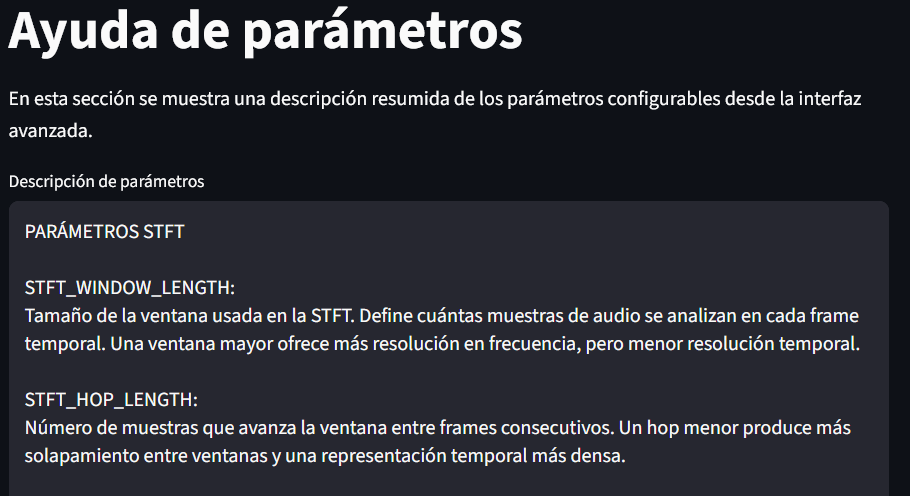
\includegraphics[width=\textwidth,height=0.55\textheight,keepaspectratio]{commons/AyudaParametros.png}
        \caption{Captura sobre la información de los parámetros}
        \label{fig:ayuda-params-gui}
    \end{subfigure}

    \caption{Entrada a la ventana de información sobre los parámetros de la configuración avanzada}
    \label{fig:informacion-parametros-gui}
\end{figure}



